\documentclass{homework}

\usepackage{tikz}
\usetikzlibrary{shapes.geometric}

\usepackage{algorithm}
\usepackage{algpseudocode}
\renewcommand{\algorithmiccomment}[1]{\hfill$\smalltriangleright$\textit{#1}}

\title{02}
\date{\DTMdate{2024-11-15}}

\newcounter{ccount}

% https://tex.stackexchange.com/a/136499
\tikzset{declare function={angleForPoly(\i,\n,\d)=360/\n*\i+\d;
                           x_radius              =\pgfkeysvalueof{/tikz/x radius};
                           y_radius              =\pgfkeysvalueof{/tikz/y radius};},
  d/.style={circle,fill,outer sep=1pt,inner sep=+0pt,minimum size=+3pt,#1},
  c/.style={insert path={(C) edge[#1,to path={circle[]}] ()}},
  a/.style={insert path={(C)+(left:x_radius+.5cm) edge[#1,<->] +(right:x_radius+.5cm)
                         (C)+(  up:y_radius+.5cm) edge[#1,<->] +( down:y_radius+.5cm)}}}
\def\nodeRot{0}
\newcommand*\poly[2][]{%
  \path (0,0) coordinate (C) [rotate/.append code={\def\nodeRot{##1}},#1]
  ++ ({angleForPoly(0,#2,0)}:x_radius and y_radius) coordinate[d] (c)
   \foreach \cnt[count=\Cnt from 0] in {1,...,#2} {
      (c) [late options={alias=c'}] (C)
      coordinate[d] (c) at ({angleForPoly(\cnt,#2,0)}:x_radius and y_radius)
      (c') edge[dashed] (c)
      \ifnum\Cnt>0 node[anchor={angleForPoly(\Cnt,#2,180+\nodeRot)},circle]
        {
          \setcounter{ccount}{\Cnt}
          \ifnum\Cnt>14\addtocounter{ccount}{1}\fi
          $\alph{ccount}$
        } \fi
   };}

\newcommand*{\polyname}{icositetragon}
\newcommand*{\polysides}{24}

\begin{document}
\maketitle

\textbf{Organisational details}
\begin{itemize}
  \item You can submit assignments up to 1 week late, however, late assignments incur a 50\% grade penalty.
  After the 1 week grace period the assignment's grade will be 0.
  \item Your submission must be a PDF.
  You can write solutions by hand and scan/photograph them, or write them using \LaTeX{} (recommended).
  If you use MS Word, you must use the equation editor for typesetting the mathematics.
  \begin{itemize}
    \item If you write solutions by hand, please make sure that the scans/pictures are of good quality (high resolution, good contrast, no blur).
    \item If your submission is not legible or is otherwise of poor quality (e.g. crossed out solutions, scribbles, \dots) we will not grade the impacted task(s).
    \item If you write code to help you solve tasks, add the code file(s) to your Moodle submission or push the code to a \emph{private} GitHub repository.
    Add \texttt{takakv} as a collaborator.
  \end{itemize}
  \item You must explicitly write out the reasoning for your solutions.
  Providing an unexplained answer will give you no points.
  \begin{itemize}
    \item Brute force is not a solution!
    \item If you write code, you must comment your code and explain what it does and why are you doing things in that way.
  \end{itemize}
\end{itemize}

\vspace*{1em}

\textbf{About help}
\begin{itemize}
  \item Homework assignments are individual work.
  While you may discuss the tasks with one-another and give hints or suggest resources, all submissions must be your own work, stem from your own thought process, and be written in your own words.
  You are not allowed to share answers, even for cross-checking.
  \item You may not use third party/online tools to solve tasks, but you may use them to check your tasks.
  \item If you use external resources\footnote{Anything that is not part of lecture or practice slides.} to help you with your homework, e.g. a CSE\footnote{Cryptography Stack Exchange} post or an article, you must properly cite that resource.
  \item If we catch you using someone else's work, we will report you for plagiarism.
  If we catch you colluding with a coursemate, we will report both of you for plagiarism.
  In both cases you will fail the course.
\end{itemize}

\newpage

\begin{task}{Scary simple}
  \autoref{fig:tetra} represents an \polyname{} in its canonical orientation.
  That is, the polygon is in its \enquote{original} position, and has not been subjected to transformations, e.g. rotation.
  The set of all symmetries of the \polyname{} forms a group under the operation $\star$.
  We define $\star$ as applying two transformations one after the other.

  A \emph{symmetry} of an object is a way of moving it so that it ends up in the space it originally occupied.
  That is, if you erase all the labels of the vertices, you would see no difference to the figure after a symmetry (or sequence of symmetries) has been applied.

  The vertices of the \polyname{} are labelled according to its rotational symmetries.
  For example, if you apply the rotation $R_b$, the point $O$ moves to $b$, the point $a$ moves to $c$, etc.

  Let the group $C_{\polysides}$ be the set of rotations:
  \[
    C_{\polysides} = \{
      \text{rotate } 0^{\circ},
      \text{rotate } 15^{\circ},
      \text{rotate } 30^{\circ},
      \dots,
      \text{rotate } 345^{\circ}
    \} = \bigl\{R_O, R_a, \dots, R_n, R_p, \dots, R_x\bigr\}.
  \]

  $C_{\polysides}$ is a cyclic group with generator $R_a$ under $\star$, and $R_O$ is the identity element.
  Indeed, applying the symmetry $R_O$ does not rotate the polygon and so its orientation remains unchanged.

  Answer the following:
  \begin{enumerate}
    \item What is the discrete logarithm of $R_t$ to the base $R_a$? \textit{(1 point)}
    \item Is the discrete logarithm problem (DLP) intractable in this group?
    In other words, do we have an efficient algorithm for solving the DLP in this group?
    Why yes/why no.
    \textit{(1 point)}
  \end{enumerate}

  \begin{figure}[h]
    \centering
    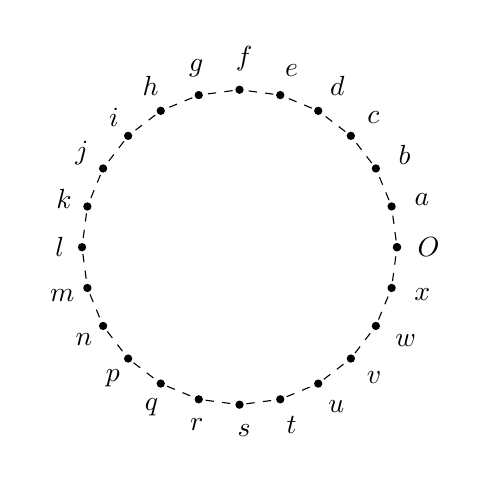
\begin{tikzpicture}[radius=2cm,>=latex]
      \poly{\polysides};
      \node (l) at (2.4,0) {$O$};
    \end{tikzpicture}
    \caption{The \polyname{}: a regular polygon with \polysides{} vertices.}
    \label{fig:tetra}
  \end{figure}
\end{task}

\begin{task}{Mechanical wonder}
  Consider the following Feistel network instantiation:
  \begin{itemize}
    \item The block size is 16,
    \item The number of rounds is 4,
    \item The round function is given by
    \[
      F_i(k_i, x) = k_i \oplus x,\qquad k_{i+1} = (k_i \ll 2) \oplus k_i
    \]
    where $\ll 2$ is a bit-shift to the left by 2 bits: bits are moved two positions to the left, only the lowest $n$ bits are kept for key-size $n$, and zeroes replace the low order shifted bits.

    Some examples of bit-shifting to the left by 2 for a key size of 4:
    \begin{itemize}
      \item $0111_2 \ll 2 = 1100$ where the actual result is $011100$ but we discard the leading $01$ due to overflow.
      We add $00$ to the right where there is now \enquote{free space} to make the block whole, i.e. of length 4.
      \item $0011_2 \ll 2 = 1100$ where we discard $00$ to the left.
      \item $1001_2 \ll 2 = 0100$ where we discard $10$ to the left.
    \end{itemize}
  \end{itemize}

  Encrypt the message $m=\texttt{1100 1010 1001 0101}$ using the Feistel instance where $k_0=\texttt{1011 0110}$.
  \textit{(1 point)}
\end{task}

\begin{task}{Playing with blocks}
  Consider the following block cipher mode of operation with block size $\lambda$ bits:
  \begin{algorithmic}[1]
    \Procedure{Encrypt}{$k, m_1||\dots||m_n$}
    \State $iv_0 \getsu \{0,1\}^\lambda$
    \For{$i = 1, \dots, n$}
      \State $c_i = \Enc_k(m_i \oplus iv_{i-1})$
      \State $iv_i = m_i \oplus c_i$
    \EndFor
    \State\Return{$(iv_0, c_1||\dots||c_n)$}
    \EndProcedure
  \end{algorithmic}

  Answer the following:
  \begin{itemize}
    \item Draw the encryption and decryption processes for at least 3 blocks.
    \textit{(1 point)}
    \item What happens to the plaintext when the 8\textsuperscript{th} bit of the second ciphertext block is flipped?
    \textit{(1 point)}
  \end{itemize}
\end{task}

\begin{task}{Complex stuff}
  For each of the following, determine the $\Oh$ complexity as closely as you can, and prove it.
  For example, if the algorithm runs in $\Oh(n^2)$, you should say $\Oh(n^2)$ and not $\Oh(n^3)$, even though both hold.

  If you prove the complexity using $n_0, c$, show the reasoning/calculations on how you obtained them and include a graph to visually confirm the values (e.g. with GeoGebra).
  Graphically finding the values will not give you full points, and you will not be able to do so during the exam.

  Here $\log$ denotes the binary logarithm, i.e. $\log_2$.

  \begin{enumerate}
    \item $f(n) = 2(n + 3)^3$ \textit{(1 point)}
    \item $f(n) = n^3 + e^{-n} - e^{2n}$ where $e \approx 2.718$ \textit{(1 point)}
    \item $f(n) = \frac{2n + \log(n) + 1}{3n}$ \textit{(2 points)}
    
    Hint: $f'(n) = \frac{1 - \ln(2n)}{n^2 \ln8}$ where $\ln = \log_e$.
  \end{enumerate}
\end{task}

\begin{task}{Reducto}
  Let $\GG$ be a cyclic, prime-order group of order $q$ with generator $g$.
  The inverse Diffie-Hellman problem is then defined as follows: given the pair $\bigl(g, g^a\bigr)$ with $a \neq 0$, find $g^{a^{-1}}$.

  Show that if you have access to an oracle which always solves the DLP, you can use it to solve the inverse Diffie-Hellman problem.
  Draw the corresponding security game.
  \textit{(2 points)}
\end{task}

\newpage

\begin{task}{What in the program?}
  Estimate the time complexity of the following algorithms in terms of $\Oh$ as closely as you can.
  For example, if the algorithm runs in $\Oh(n^2)$, you should say $\Oh(n^2)$ and not $\Oh(n^3)$, even though both hold.
  You can assume that addition, subtraction, multiplication, and division are $\Oh(1)$ operations.
  Explain your reasoning.

  \begin{enumerate}
    \item \textit{(1 point)}
    \begin{algorithmic}[1]
      \Procedure{loopy}{$n$}
      \State $t \gets 0$
      \For{$i = 0, \dots, n-1$}
        \For{$j = 0, \dots, n-1$}
          \For{$k = 0, \dots, n-1$}
            \State $t \gets t + i \cdot j \cdot k$
          \EndFor
        \EndFor
      \EndFor
      \State\Return{t}
      \EndProcedure
    \end{algorithmic}

    \item \textit{(1 point)}
    \begin{algorithmic}[1]
      \Procedure{recursive}{$n$}
      \If{$n \leq q$} 
        \Return{$n$}
      \EndIf
      \State\Return{\Call{recursive}{$n - 1$} + \Call{recursive}{$n - 2$}}
      \EndProcedure
    \end{algorithmic}

    \item \textit{(2 points)}
    \begin{algorithmic}[1]
      \Procedure{mixed}{$n$}
      \State $s \gets 0$
      \For{$i = 0, \dots, n-1$}
        \State $s \gets s + 1$
        \State $k \gets n$
        \While{$k > 0$}
          \State $k \gets \lfloor k/2 \rfloor$
          \Comment{Floored division, i.e. discard the fractional part.}
          \State $s \gets s + k$
        \EndWhile
      \EndFor
      \State\Return{s}
      \EndProcedure
    \end{algorithmic}
  \end{enumerate}
\end{task}

\newpage

\begin{task}{Generating solutions (bonus)}
  Show that if you have access to an oracle which always solves the computational Diffie-Hellman problem, you can use it to solve the inverse Diffie-Hellman problem.
  Draw the corresponding security game.
  \textit{(2 points)}

  Hint: you are not required to send the correct generator $g$ to the oracle.
\end{task}

\end{document}
